\documentclass[10pt,a4paper,twoside]{article}
\usepackage{latexsym}      % needed math symbols
\usepackage{hyperref}
\hypersetup{
 colorlinks=true,
 citecolor=blue,
 linkcolor=blue,
 urlcolor=blue,
 pdfpagemode=UseNone,
 pdfstartview=FitH}
\usepackage{graphicx}      % for importing eps figures
\usepackage{amsmath}       % for advanced math symbols
\usepackage[affil-sl]{authblk} 			% found in preprint bundle package, http://ctan.org/pkg/preprint
\usepackage[margin=2.5cm]{geometry} % paper and margin formats as set by SPP
\usepackage{subfig}

\parindent 0.5cm    % paragraphs indent
\topmargin=-2cm

% SPP details
\newcommand{\spp}{38\textsuperscript{th}}
\newcommand{\sppvenue}{Legazpi City, Albay}
\newcommand{\sppdate}{3--6 June 2020}


% title style
\newcommand*{\TitleFont}{\bfseries \Large }

% authblk style
\newcommand{\authorsep}{,\negmedspace}
\newcommand{\lastauthorsep}{}
\makeatletter
\renewcommand\AB@authnote[1]{{\textsuperscript{\normalfont#1}\ }}
\renewcommand\Authsep{}
\renewcommand\Authands{and }
\renewcommand\Authfont{\small {\bfseries}}
\renewcommand\Affilfont{\small	\itshape}
\setlength{\affilsep}{5pt}
\makeatother
\newcommand{\corremail}{\rm Corresponding author:~}

% remove date
\date{}

% for abstract style
\makeatletter
\newbox\abstract@box
\renewenvironment{abstract}
   {\global\setbox\abstract@box=\vbox\bgroup
     \hsize=\textwidth\linewidth=\textwidth
    \vspace{-2em}
		\small
		%\begin{center}
		{\hspace{1.2em}\bfseries \abstractname\vspace{.0em}\vspace{\z@} }%
		%\end{center}
    \quotation}
  {\endquotation\egroup}
\expandafter\def\expandafter\@maketitle\expandafter{\@maketitle
	\ifvoid\abstract@box\else\unvbox\abstract@box\if@twocolumn\vskip1.5em\fi\fi}
\makeatother
\providecommand{\keywords}[1]{\vspace{.5em}\noindent \mdseries{{Keywords:}} #1}
\providecommand{\DOI}[1]{\vspace{#1\baselineskip}}
\providecommand{\dateline}[1]{\vspace*{-1\baselineskip}\normalsize Submitted: #1\vspace*{-1.5\baselineskip}}

% for section formatting style
\makeatletter
\renewcommand\section{\@startsection
   {section}{1}{0pt}%
   {-\baselineskip}%
   {0.1\baselineskip}%
   {\normalfont\large\bfseries}}%
\renewcommand\subsection{\@startsection
   {subsection}{1}{0pt}%
   {-\baselineskip}%
   {0.1\baselineskip}%
   {\normalfont\bfseries}}%
\makeatother
\renewcommand\thesection{\arabic{section}}

% for the figure and tables, captions
\usepackage{booktabs}
\usepackage{dcolumn}
\newcolumntype{d}[1]{D{.}{.}{#1}}

\usepackage{caption}
\captionsetup[table]{position=above,font={rm,small}}
\captionsetup[figure]{font={rm,small}}

% for citations formatting style
\usepackage[numbers,square,sort&compress]{natbib}
\setlength\bibsep{1pt}

%%for first page styling 
\providecommand{\articlenum}[0]{}
\usepackage{fancyhdr}
\fancypagestyle{titlestyle}
{
\renewcommand{\headrulewidth}{0pt}
\renewcommand{\footrulewidth}{0.1pt}
\fancyhf[l]{}
\fancyhf[c]{ }
\fancyhf[r]{ }
\fancyfoot[l]{}
\fancyfoot[c]{\href{https://paperview.spp-online.org/proceedings/issue/archive}{Proceedings of the Samahang Pisika ng Pilipinas} \\ \href{https://paperview.spp-online.org/proceedings/issue/view/SPP-2020}{\spp\,Samahang Pisika ng Pilipinas Physics Conference}\\ \sppvenue, \sppdate \\ \articlenum 1}
\fancyfoot[r]{}
}

% styling for the second page onwards
\renewcommand{\headrulewidth}{0pt}
\renewcommand{\footrulewidth}{0.1pt}
\fancyhf[l]{}
\fancyhf[r]{}
\fancyhf[c]{}
\fancyfoot[l]{}
\fancyfoot[c]{\href{https://paperview.spp-online.org/proceedings/issue/archive}{Proceedings of the Samahang Pisika ng Pilipinas}  \\ \href{https://paperview.spp-online.org/proceedings/issue/view/SPP-2020}{\spp\,Samahang Pisika ng Pilipinas Physics Conference}\\ \sppvenue, \sppdate \\ \articlenum \thepage}
\fancyfoot[r]{}
\pagestyle{fancy}

% other packages and macros
\usepackage{bm}
\renewcommand{\vec}[1]{\text{\bfseries #1}}

\usepackage{physics}
\usepackage{amsfonts}
\usepackage{changes}
\usepackage{graphicx}
\graphicspath{{images/}}
\newcommand{\snrseg}{SNR$_{\mathrm{seg}}$}

%\makeatletter
%\@namedef{Changes@AuthorColor}{red}
%\colorlet{Changes@Color}{red}
%\makeatother

%  Editorial staff will uncomment the next line
% \providecommand{\artnum}[0]{XX-XX}
% \renewcommand{\articlenum}[0]{SPP-\the\year-\artnum-}

\begin{document}

\title{\TitleFont Compressively sampled speech: How good is the recovery?}

\author[*\negthickspace]{Kenneth V.~Domingo}
\author[ ]{Maricor N.~Soriano
\lastauthorsep}
\affil[ ]{National Institute of Physics, University of the Philippines, Diliman, Quezon City, Philippines}
\affil[*]{\corremail{kdomingo@nip.upd.edu.ph} }


\begin{abstract}
\noindent
Modern signal acquisition technologies are made possible by the Nyquist-Shannon sampling theorem (NST). However, this paradigm is extremely wasteful as the signal is compressed before storing it by systematically discarding imperceptible information. Compressive sensing (CS) aims to directly sense the relevant information. Current literature focus either on formulating more computationally-efficient algorithms, or methods which improve the reconstruction quality. In this paper, we quantify the reconstruction quality of compressively sampled speech with a perceptually intuitive metric---the Perceptual Evaluation of Speech Quality (PESQ)---and with the standard average segmental SNR (\snrseg). The quality of recovery of compressively sampled speech evaluated using PESQ is dependent on the compression ratio, and independent of the number of subbands used to represent the signal in the spectrogram domain.

\keywords{compressive sensing, signal processing, spectrogram}

\end{abstract}

\maketitle
\thispagestyle{titlestyle}

\section{Introduction}\label{sec:intro}
Conventional sensing devices are based on the Nyquist-Shannon sampling theorem (NST), which states that given a signal's bandwidth, one can capture all the pertinent information about that signal if it is sampled at a rate at least twice the signal's highest frequency component. After sampling, information is compressed by exploiting the signal's natural compressibility in some transform domain. For most applications, this tried-and-true method of sampling and systematically discarding the imperceptible information is acceptable. However, in situations when transmission bandwidth and/or storage comes at a premium, this process is highly wasteful. Cand\'{e}s et al. \cite{Candes2006} and Donoho et al. \cite{Donoho2006} independently pioneered compressive sensing (CS), which could directly sample the portions of a signal that would otherwise survive the compression stage in conventional sampling. In this new sampling paradigm, we consider the linear model of signal acquisition

\begin{equation}\label{eq:cesa}
	y_k = \vec{x} \cdot \vec{a}_k
\end{equation}

The signal vector $\vec{x} \in \mathbb{R}^n$ is correlated with the basis waveforms $\vec{a}_k$ to yield a compressed information vector $\vec{y} \in \mathbb{R}^m$, where $m \ll n$. This causes the task of recovering $\vec{x}$ from $\vec{y}$ infeasible since there exist an infinite number of candidate solutions $\bm\hat{\vec{x}}$ which satisfy \eqref{eq:cesa}. This can be circumvented by enforcing sparsity and incoherence constraints \cite{Candes2008b} based on models of natural signals. The process of reconstruction can then be recast into a general minimization problem

\begin{equation}\label{eq:minl1}
	\min_{\vec{x}} \norm{\vec{x}}_1 \quad \textrm{subject to} \quad \vec{A}\vec{x} = \vec{y}
\end{equation}

\noindent where $\norm{\vec{x}}_1$ denotes the $\ell_1$ norm of $\vec{x}$. This problem can be solved with various algorithms.

Romero et al. \cite{Romero2016} performed compressive sensing of images in the Fourier domain and showed that it could be used to increase the signal-to-noise ratio of a signal. In the realm of audio signals, Mathew \& Premanand \cite{Mathew2016} constructed sensing matrices using a Gaussian-Logistic map. Theirs was one of the first studies which use chaotic maps instead of random sequences. Through evolutionary algorithms such as differential evolution, direct reconstruction of CS signals could also be attained in the temporal domain \cite{Andras2018}. With audio recordings containing speech, however, the process is not as straightforward. Such signals typically use sampling rates of $\sim 10^{3}$ Hz, so it is necessary to process them in slices, in the same way that large images can be processed in patches. Low et al. \cite{Low2018} performed this process by representing a signal in the spectrogram/modulation domain and applying the desired CS algorithm per sampling window.

In this paper, we perform compressive sensing of audio signals containing speech, and quantify the reconstruction quality using the Perceptual Evaluation of Speech Quality (PESQ). Current metrics for evaluating reconstructed speech quality which are based on the statistical properties of the signal, such as mean-squared error (MSE) and peak signal-to-noise ratio (PSNR), are non-intuitive and have undefined bounds. The former indicates that it is difficult to gauge and compare the quality of a signal with an MSE value of 0.1, compared to another with an MSE value of 0.01 without explicitly observing them, while the latter yields values that may change depending on the length of the signal or of the sampling window, implying some degree of scale-variance. On the other hand, PESQ is an objective speech quality assessment primarily modeled after an older subjective scoring system, essentially emulating how a person might rate a signal from 1 (bad) to 5 (excellent) given a clean reference signal \cite{pesq}. Thus, it is easy to gauge a signal's quality based on the PESQ value without actually observing the signal itself. Additionally, the average segmental signal-to-noise ratio (\snrseg), which is commonly used in evaluating window-sampled audio reconstruction quality, was also used. However, its values are non-intuitive since it is also based on the statistical properties of the signal. Consequently, its value also varies with the number of sampling windows, which is an important variable to be explored in this paper. Furthermore, we are also interested in how changing the compression ratio (CR) and/or number of sampling windows affect the reconstruction quality in terms of these two metrics. We adopt the processing workflow of Low et al. while varying the length and number of sampling windows, as well as the CR. In contrast with Mathew et al., we stick with the usual sensing matrices derived from i.i.d.~uniform random samples. In an earlier work \cite{Domingo2019}, we compared common algorithms in terms of computation time and reconstruction quality, and showed that LASSO strikes a balance between these two. We use this algorithm in this paper to perform the CS reconstruction.


\section{Methodology}\label{sec:metho}

\subsection{Obtaining \& preprocessing the test signals}\label{ssec:timit}
The test signals used in this paper were obtained from the TIMIT Acoustic-Phonetic Continuous Speech Corpus \cite{timit}, which contains speech recordings, in WAV format, of English speakers separated by region, sex, and spoken sentence. All recordings have a sampling rate of 16 kHz and are 3 seconds long on average. This was then downsampled to 8 kHz to reduce the number of sampling windows needed, and also because the PESQ algorithm only applies to 8 kHz signals.

\subsection{Transforming to a sparse domain}\label{ssec:sparse}
The first requirement for CS is that a signal should be transformed to a domain where it can be represented sparsely. In the case of recorded speech, the most appropriate domain would be the modulation domain, otherwise known as its spectrogram. First, we define the length of the sampling window and the percent overlap between adjacent windows, and divide the signal into frames using this sliding window. We then multiply each frame by a window function, typically a Hann window, defined as

\begin{equation}\label{eq:hann}
	w[n] = \sin[2](\frac{\pi n}{N}), \quad 0 \leq n \leq N
\end{equation}

\noindent where $N+1$ is the length of the window. Finally, we take the Fourier transform of each frame. The entire process is also called a short-time Fourier transform and can be summarized as

\begin{equation}\label{eq:stft}
	X(\omega, p) = \sum_{p=0}^{P-1} x[p] w[p - kR] e^{-i\omega p}
\end{equation}

\noindent where $x[p]$ indicates the $p$th signal frame, $w[n-k]$ is the window function with hop size $R$, $k$ is the time index, and $\omega$ is the frequency. Figure~\ref{fig:original} shows a test signal in the temporal domain (top) and its corresponding spectrogram (bottom) with a 25 ms sampling window and 75\% frame overlap.

\subsection{Compressive sensing}\label{ssec:cs}
The second requirement of CS is that the sensing matrix should be incoherent with the sparse basis. Typically, random samples are drawn that are distributed uniformly to simulate compressive measurements. We define an index sequence $\xi$ corresponding to a random subset of $m$ samples from the signal. The compressed signal vector can be defined as $\vec{y} = \vec{x}_\xi$, and the sensing matrix $\bm\Phi \in \mathbb{R}^{m \times n}$ can be constructed by stacking the columns of a discrete cosine transform (DCT) matrix indexed by $\xi$. This sensing matrix can then be used for all the frames. After multiplying the frame with a window function, instead of directly taking the frame's Fourier transform, we can now perform reconstruction of the signal from the compressive measurements. The objective of LASSO is

\begin{equation}\label{eq:lasso}
	\min_{\vec{x}} \frac{1}{2m} \norm{\vec{y} - \bm\Phi \vec{x}}_2^2 + \alpha\norm{\vec{x}}_1
\end{equation}

\noindent where $m$ is the number of samples, and $\alpha$ is the $\ell_1$ regularization parameter.

\subsection{Reconstruction evaluation}\label{ssec:eval}
Reconstruction quality was evaluated using PESQ, which is a full-reference, perceptually intuitive scoring system which models the obsolete mean opinion scores (MOS). Due to the complexity of the algorithm, we refer the reader to Sec.~10 of the PESQ manual \cite{pesq} for an in-depth discussion.

The \snrseg~, defined as

\begin{equation}\label{eq:snrseg}
	\mathrm{SNR_{seg}} = \frac{10}{B} \sum_{b=0}^{B-1} \log_{10} \frac{\sum_{i=Nb}^{Nb+N-1} x_i^2}{\sum_{i=Nb}^{Nb+N-1} \qty(x_i - \hat{x}_i)^2}
\end{equation}

\noindent was also used, where $N$ is the frame length, $B$ is the number of frames, $x_i$ are  the original signal samples, and $\hat{x}_i$ are the reconstructed signal samples.


\section{Results and Discussion}
A test signal was chosen at random from the TIMIT corpus, specifically the \texttt{DR8/MJLN0/SA1.wav} file. This indicates that the speaker was from dialect region 8 (nomadic), was male with speaker code \texttt{JLN0}, and spoke sentence code \texttt{SA1}, which reads ``She had your dark suit in greasy wash water all year''. After downsampling, the signal was compressively sampled with a CR of 40\% using 1024 frames and 75\% frame overlap. The optimal regularization $\alpha$ was determined automatically via 5-fold cross validation, and the reconstruction result is shown in Fig.~\ref{fig:recovered}. Qualitative comparison in the temporal domain shows that the waveforms of the original and reconstructed are similar; in the modulation domain, the dynamic range decreased, but the dominant frequencies can still be observed. Evaluating the PESQ and \snrseg~yields values of 2.50 and 0.07, respectively. By inspection of the PESQ value alone, we can tell that the reconstructed signal quality is slightly below average. This distinction cannot be made for the \snrseg~since its bounds are not clearly defined.

Next, the error maps for the signal were generated by compressively sensing the signal and evaluating the metrics for varying CR $m/n \in [0.1, 0.9]$ (in increments of 0.1) and number of frames/subbands $\in \qty{128, 256, 512, 1024}$, while keeping the frame overlap constant. Figure \ref{fig:pesq-snr} shows the PESQ map (left) and the \snrseg~map (right). The former exhibits sensitivity to the CR and achieves a value of 4.0 (good) at around 70\% compression. The latter tells a different story: it shows sensitivity towards the number of frames/subbands (as it is an \textit{average} metric) with some additional degradation at lower CR, and achieves a maximum value of 0.08 at around 1024 frames.


\begin{figure}[tbp]
	\centering
	\subfloat[Original]{\makebox[0.46\textwidth]{{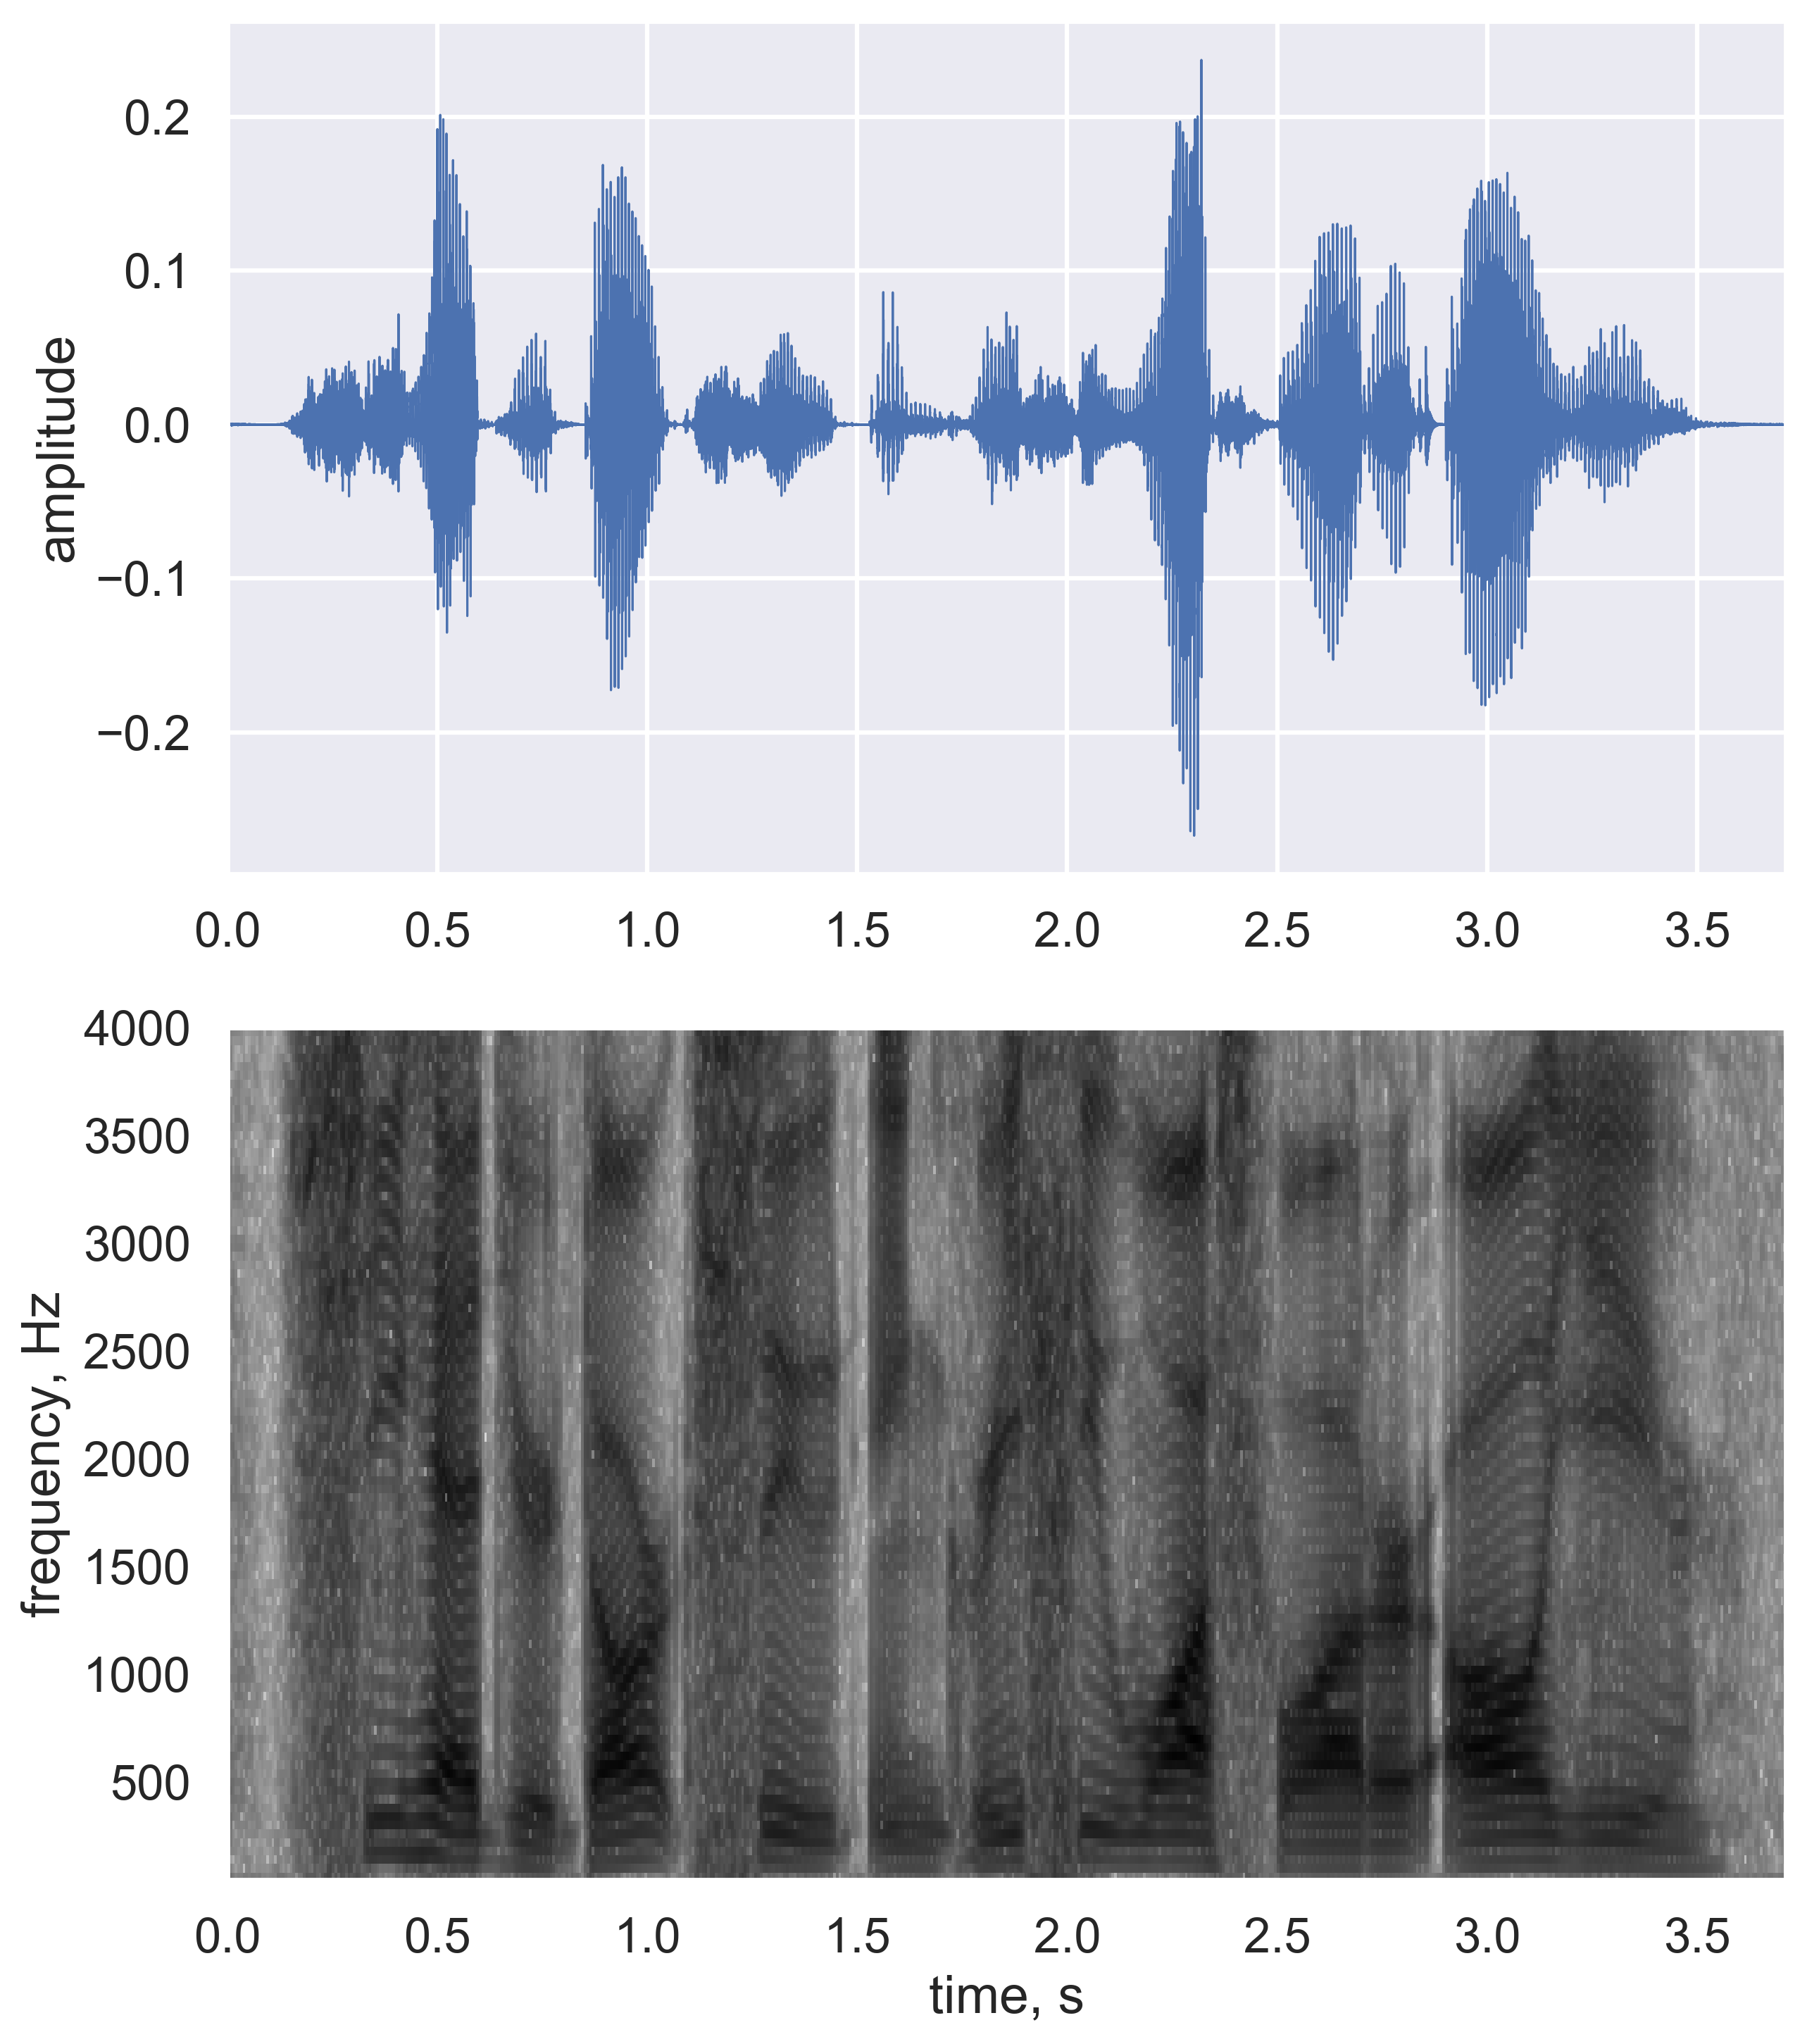
\includegraphics[width=0.46\textwidth]{original.png}\label{fig:original}}}}
	\quad % or other spacing between figures
	\subfloat[Recovered]{\makebox[0.46\textwidth]{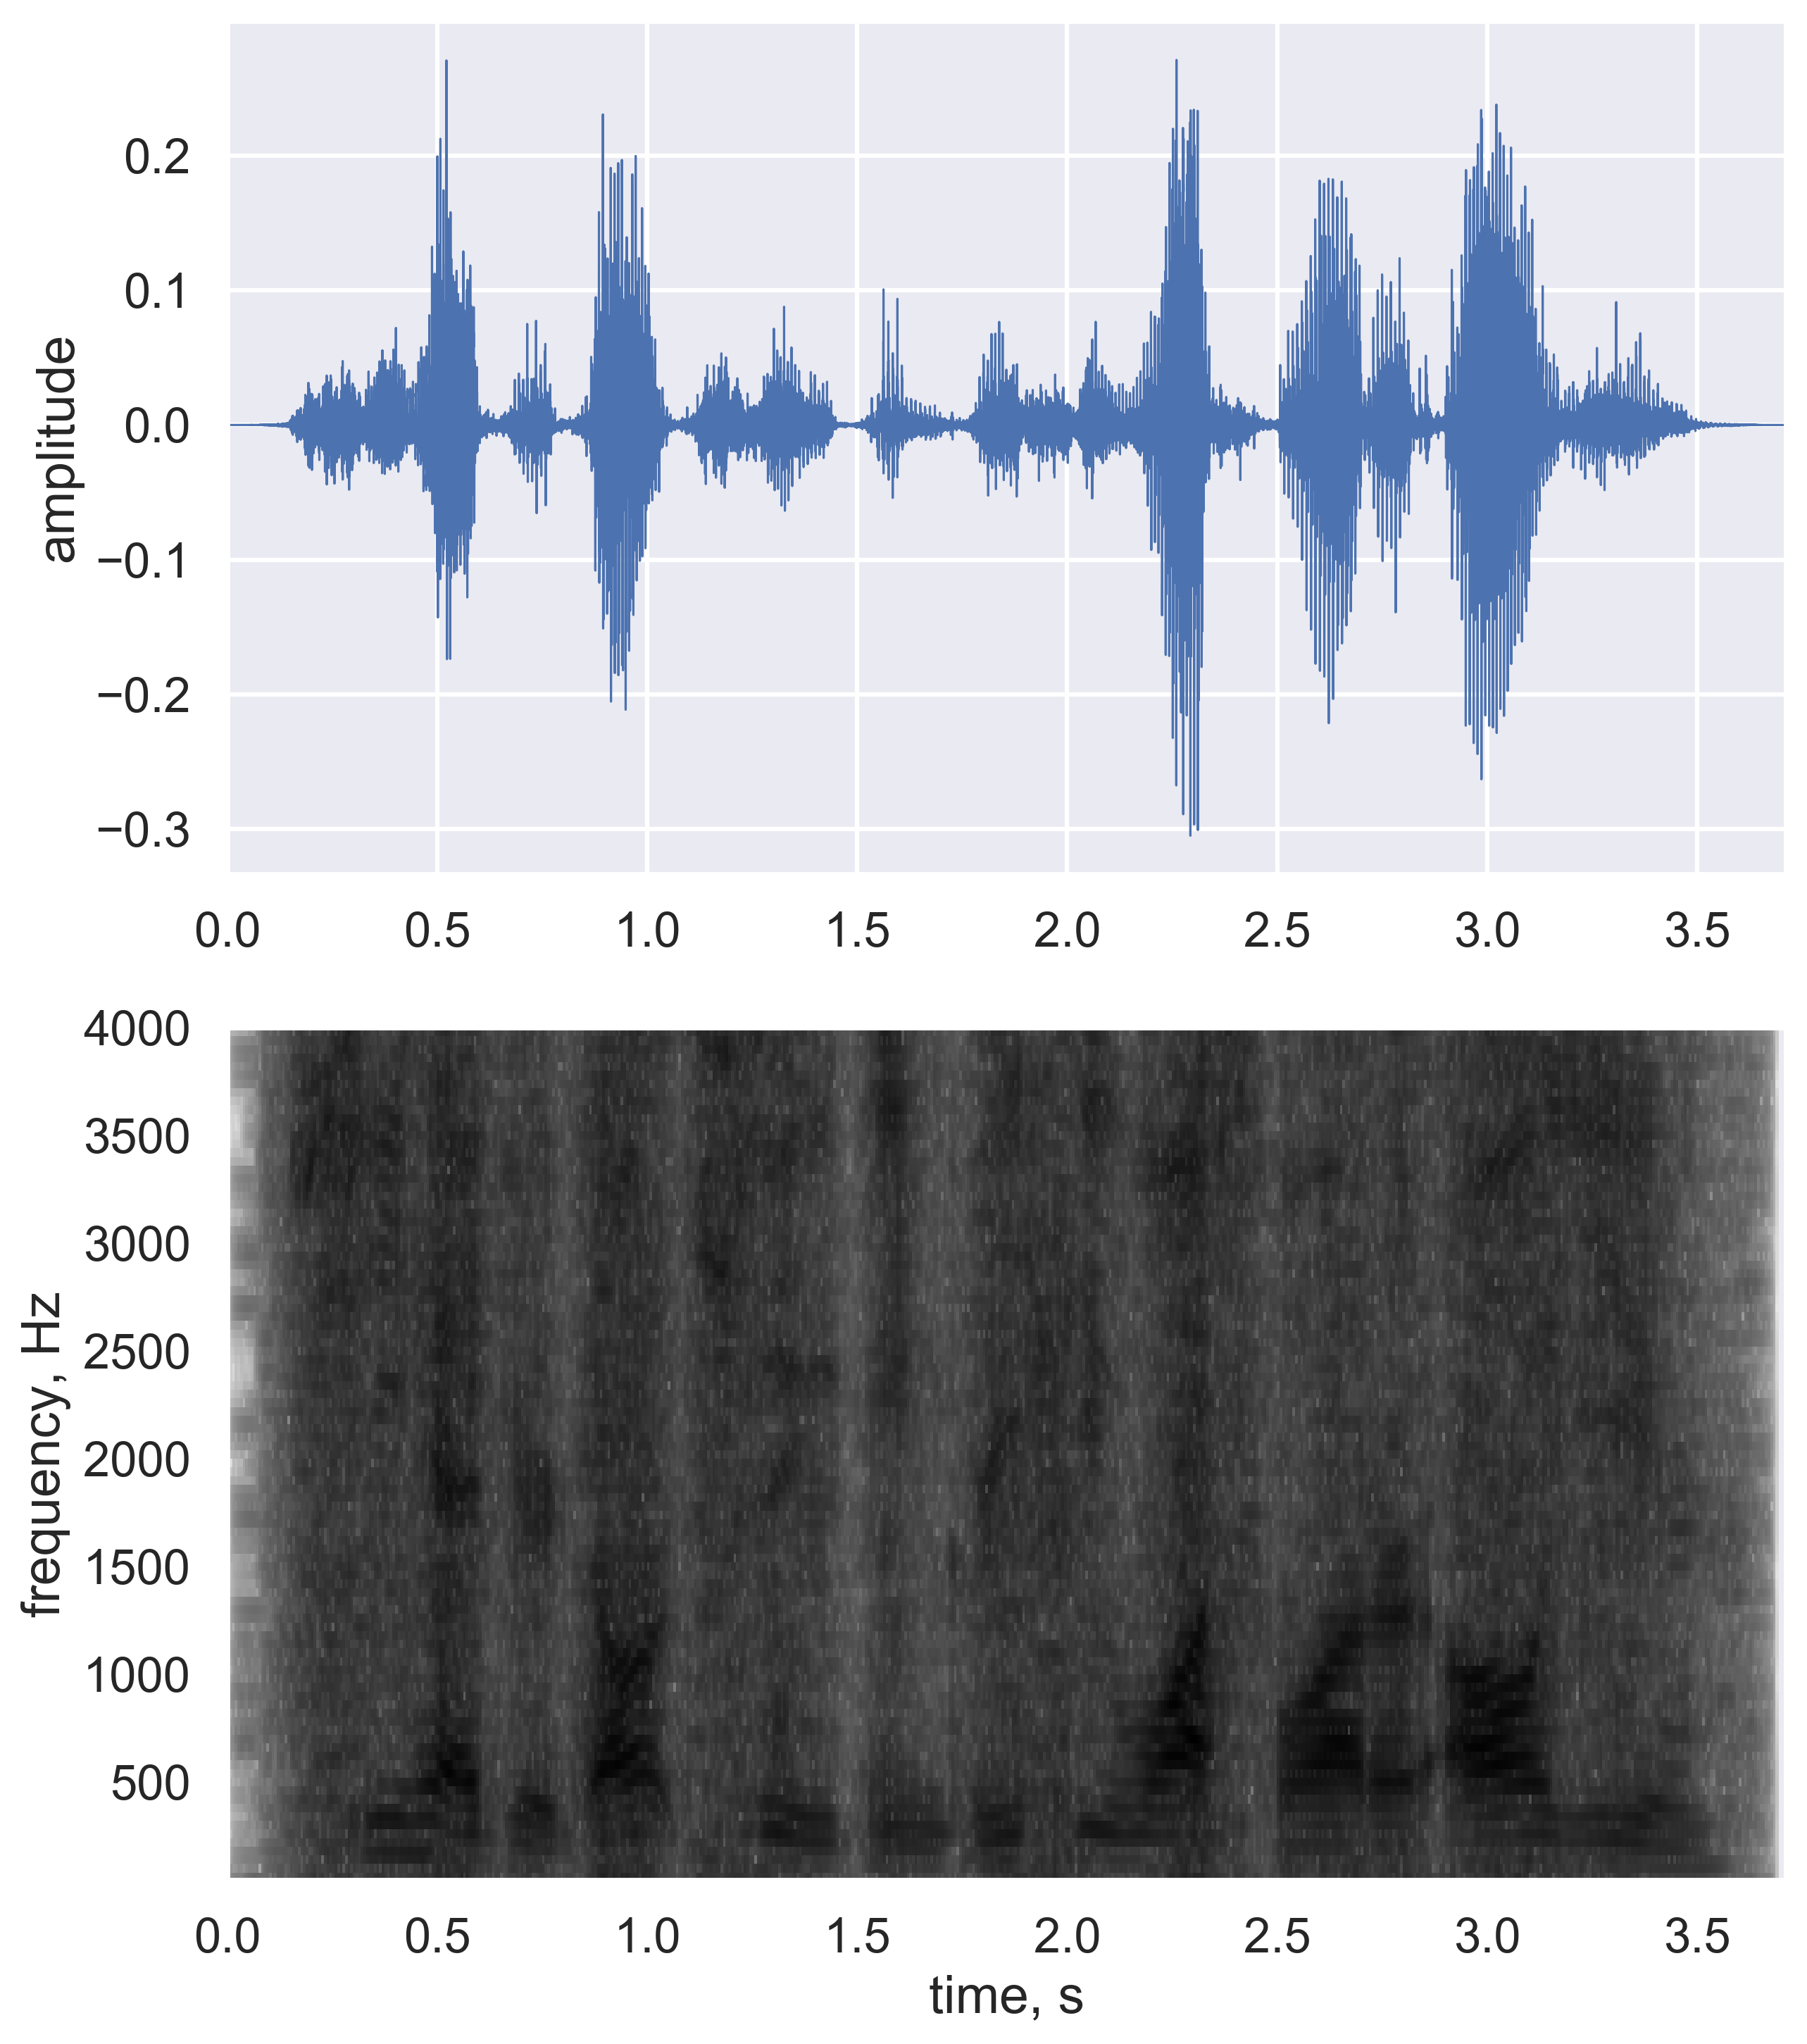
\includegraphics[width=0.46\textwidth]{recovered.png}\label{fig:recovered}}}
	\caption{Test speech signal obtained from the TIMIT speech corpus with the (a) original signal, and (b) reconstructed signal from compressive measurements. The top row is the representation in the time domain, while the bottom row is the spectrogram representation (25 ms sampling window with 75\% overlap). The signal reads ``She had your dark suit in greasy wash water all year''.}\label{fig:spectrogram}
\end{figure}

\begin{figure}[tb]
	\centering
	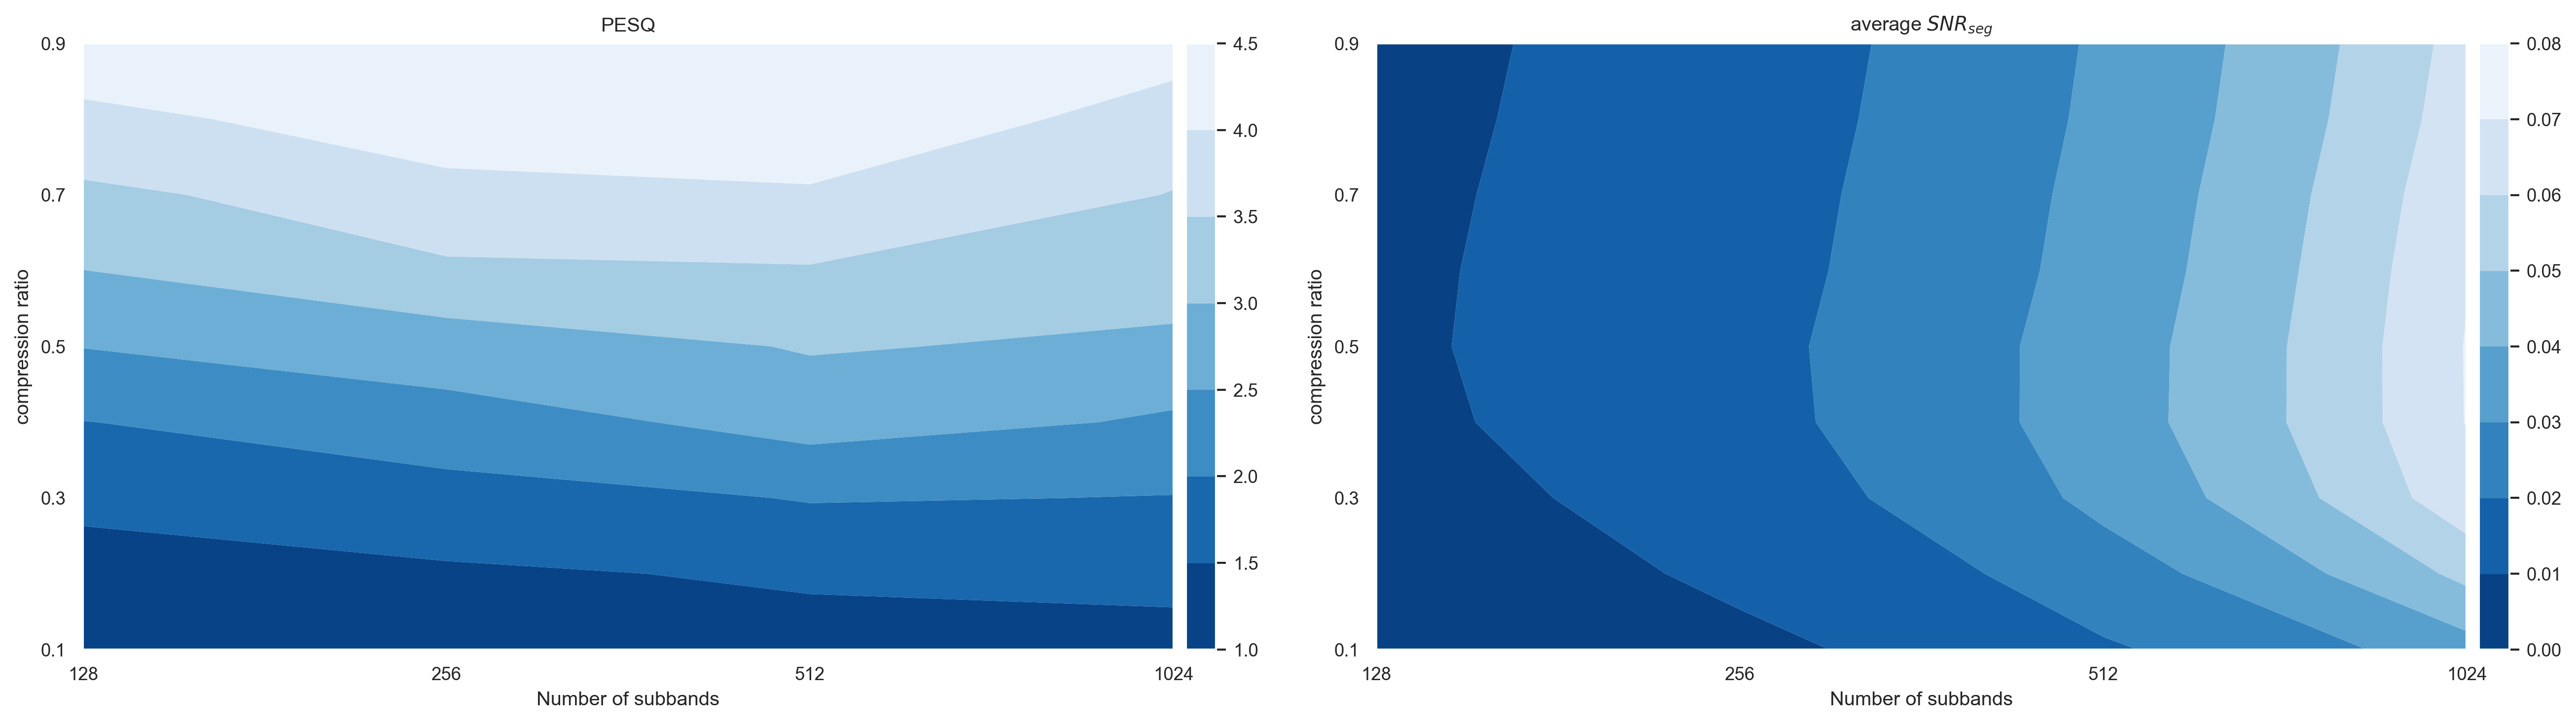
\includegraphics[width=\textwidth]{metrics.png}
	\caption{Two most commonly used metrics in evaluating quality of reconstructed speech recordings. PESQ is sensitive to the signal compression (left), while the \snrseg~is sensitive to the number of subbands (right).}
	\label{fig:pesq-snr}
\end{figure}


\section{Conclusions}
The reconstruction quality of compressively sampled audio signals containing speech recordings was described by varying two distinct factors, namely, the compression ratio and number of subbands/sampling windows. Evaluation of a perceptually intuitive metric such as PESQ shows that it is sensitive to changes in compression but independent of the number of spectrogram subbands, wherein a compression ratio of 60\% is sufficient to yield an average (3.0) PESQ score. On the other hand, evaluation of a statistically-based metric such as \snrseg~shows that it is sensitive to changes in the number of subbands used to represent the signal in the spectrogram domain, where the use of more frames yields a higher \snrseg~score.


\bibliographystyle{spp-bst}
\bibliography{bibfile}

\end{document}